\chapter{Results}\label{chap:evaluation_and_results}
This chapter presents the outcomes of the two primary areas of investigation in this thesis: the development of the Study Buddy RAG chatbot prototype, and the assesment of the implementation of low-rank approximation on the BART model. This chapter is structured to provide a comprehensive overview of the findings, highlighting the impact of document insertion on the chatbot's performance and the effectiveness of low-rank approximation in optimizing the BART model.

The first section focuses on the Study Buddy RAG chatbot prototype, detailing the internal functionality tests and case studies that assess the impact of inserting relevant documents on the chatbot's response quality. The evaluation emphasizes the improvements in accuracy, relevance, and response quality that result from enhancing the chatbot with additional context.

The second section addresses the low-rank approximation of the BART model. It examines the fine-tuning process, presents ROUGE scores to evaluate summarization performance, and discusses the computational efficiency gains achieved through low-rank approximation. Additionally, the section includes a comparison of generated summaries at various approximation ranks to illustrate the trade-offs between model compression and performance retention.

\section{RAG Chatbot}
The primary goal of developing the Study Buddy RAG chatbot prototype was to gain hands-on experience with working with LLMs and their application in real-world language processing tasks. %The evaluation metrics used to assess the chatbot focused on its internal performance and functionality rather than user testing:

The evaluation of the Study Buddy chatbot involved querying the chatbot both before and after inserting relevant documents. The aim was to observe how the inclusion of additional context impacts the chatbot's performance in terms of accuracy, relevance, and response quality. This internal testing was done to verify that the chatbot was ready for potential future scalability and subsequent testing by multiple users.

\subsection{Functionality Testing}
The functionality of the chatbot was tested by ensuring that all components (retriever, generator, and PDF uploader) worked seamlessly together. This involved verifying the following:

\begin{itemize}
    \item \textbf{PDF Uploader:} Successfully uploading PDF documents and storing them in the Astra DB Vector Store.
    \item \textbf{Retriever Component:} Accurately retrieving relevant documents based on user queries.
    \item \textbf{Generator Component:} Generating coherent and contextually relevant responses using the GPT-4 model.
    \item \textbf{Integration:} Ensuring that the retriever and generator components integrate smoothly to provide comprehensive responses.
\end{itemize}
The Study Buddy chatbot successfully passed all functionality tests, demonstrating that the components worked together seamlessly to provide accurate and contextually relevant responses to user queries when relevant documents were inserted. Section \ref{document_insertion} provides examples of how the chatbot was tested before and after inserting relevant documents.

\subsection{Case Study: Impact of Document Insertion on Response Quality}\label{document_insertion}
A series of specific queries were made to the Study Buddy chatbot before and after inserting a set of relevant documents. The goal was to observe changes in the quality of responses. The queries were related to complex topics that required detailed and specific information.

\textbf{Example Query 1:}
The first query was related to the topic of "orthogonal matrices" and involved asking the chatbot to explain the properties of orthogonal matrices.
\begin{itemize}
    \item \textbf{Before Document Insertion:} The chatbot provided a general and correct overview of the topic.
    \begin{figure}[H]
        \centering
        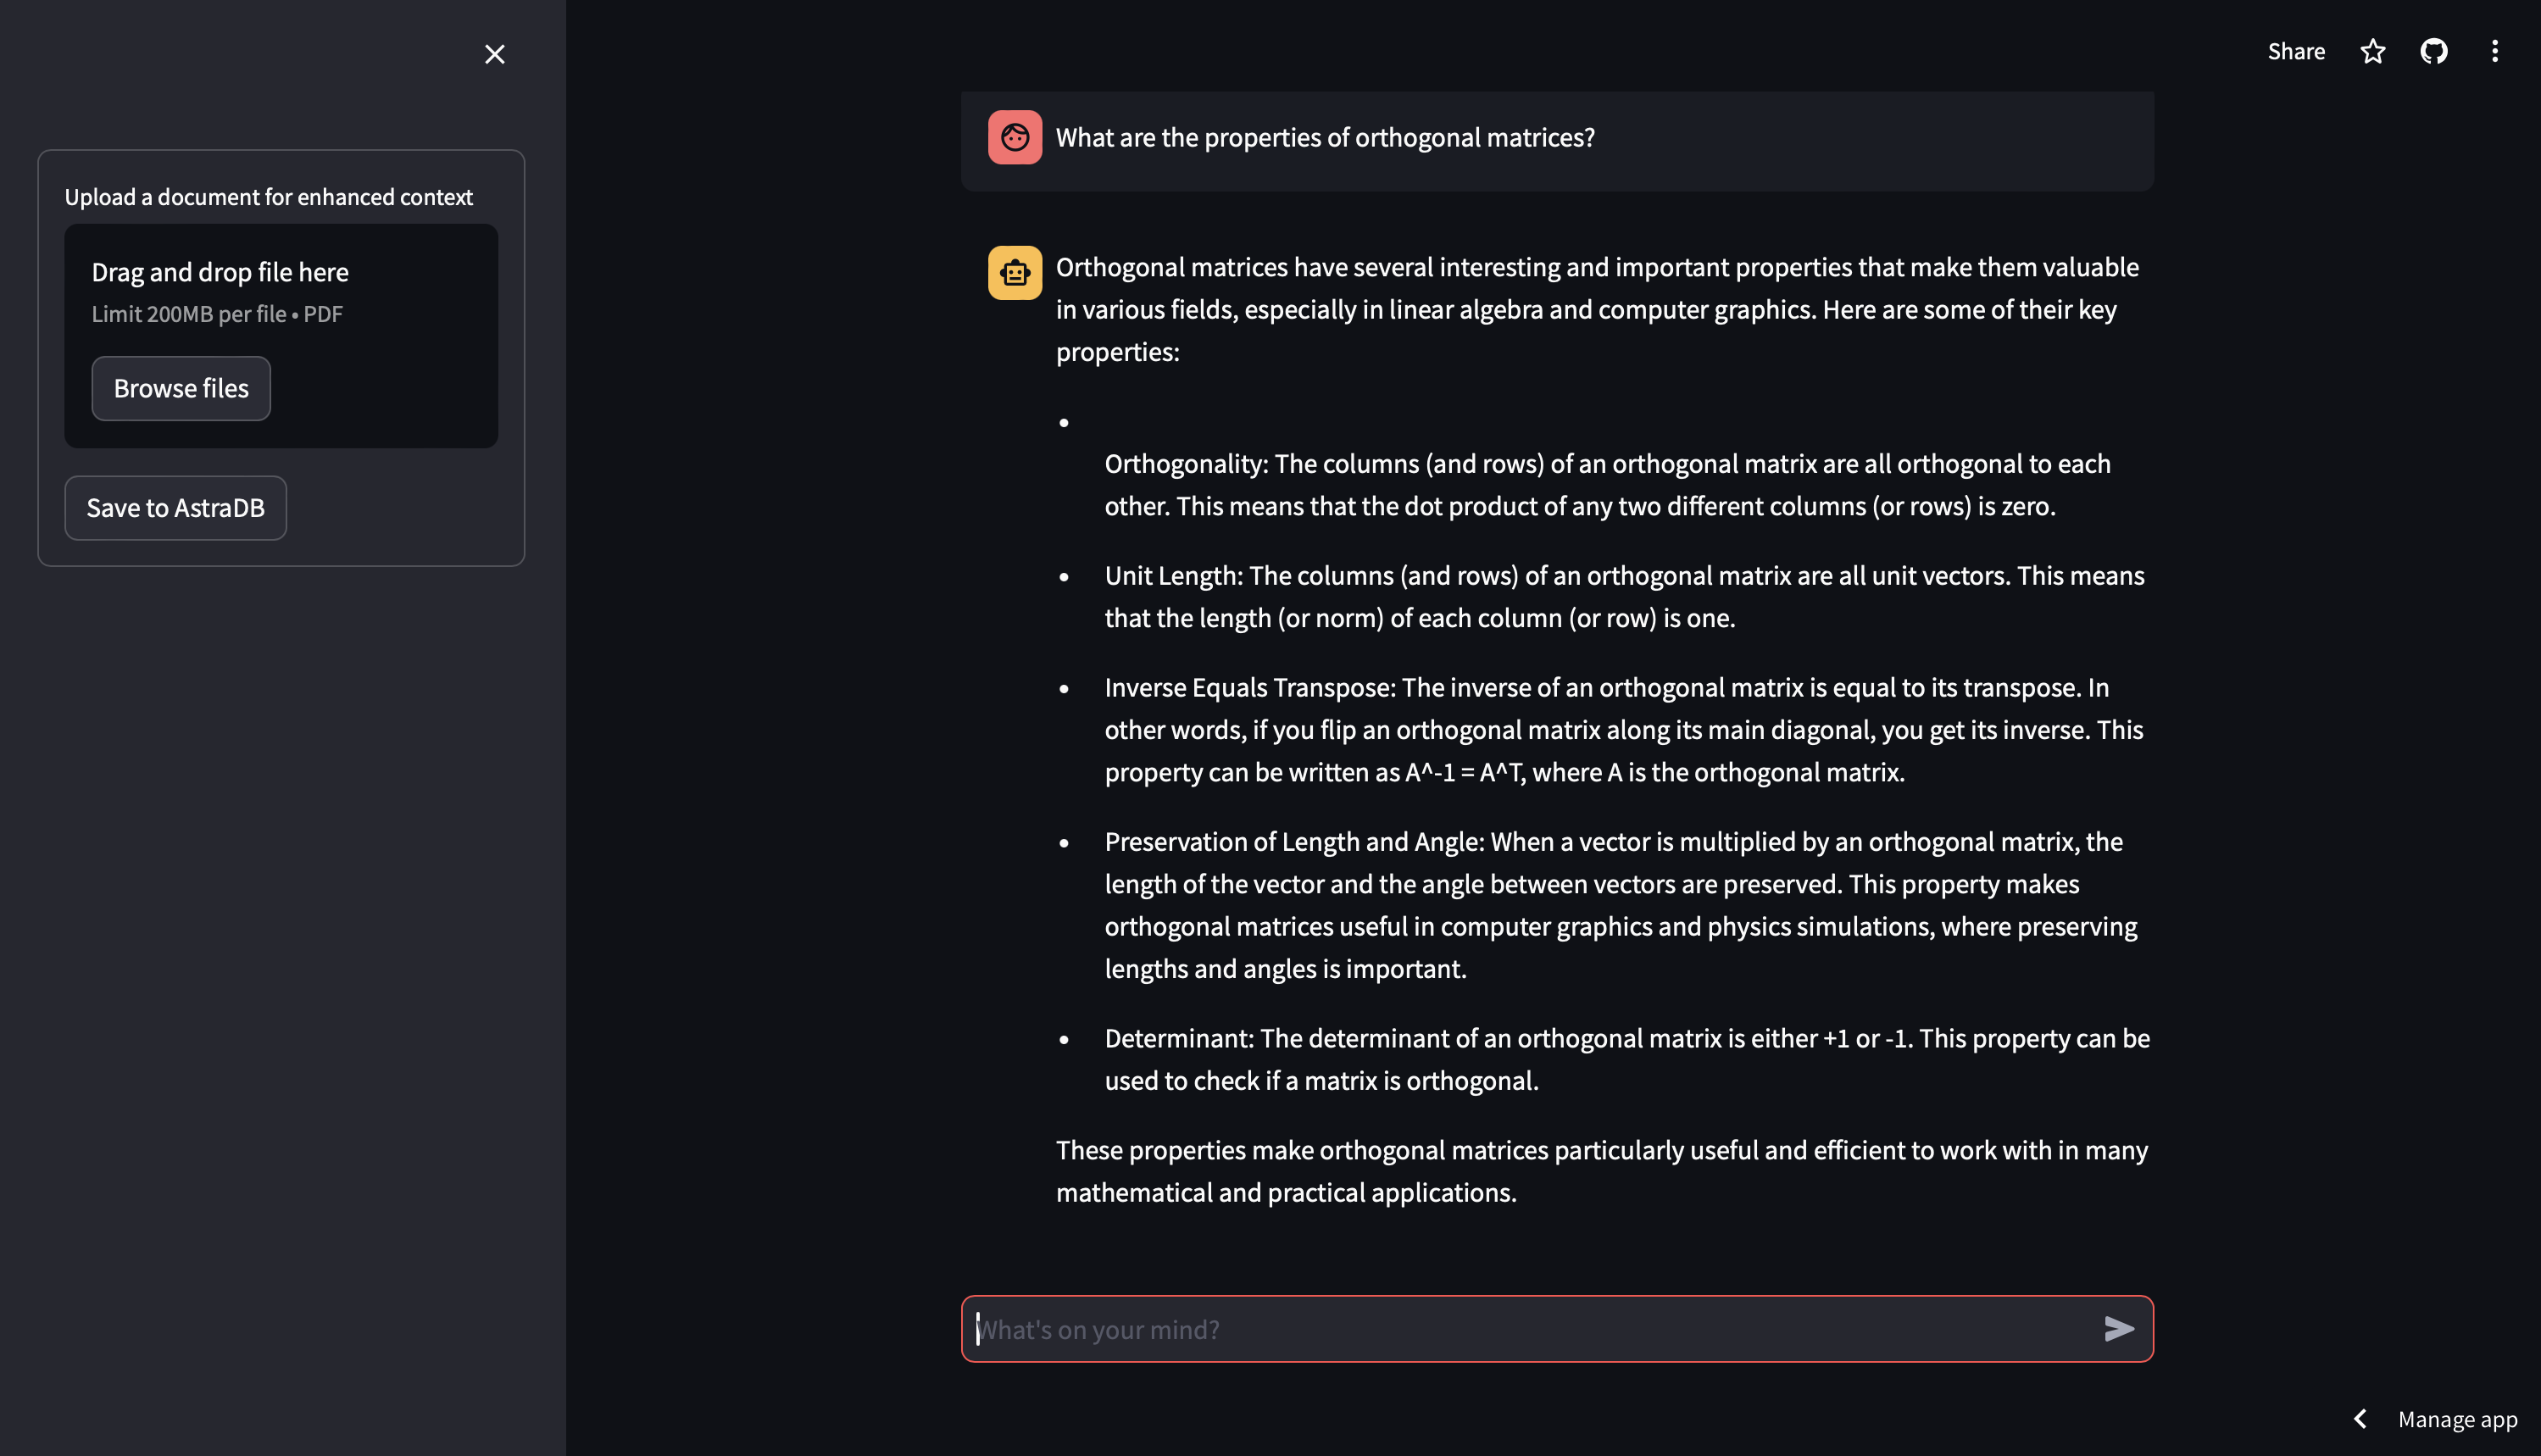
\includegraphics[width=0.8\textwidth]{figs/BeforeOrthogonal.png}
        \caption{Response before insertion of lecture slides on orthogonal matrices}
        \label{fig:before_orthogonal_matrices}
    \end{figure}
    \item \textbf{After Document Insertion:} The chatbot referenced specific information from the uploaded documents, while providing an accurate response.
    \begin{figure}[H]
        \centering
        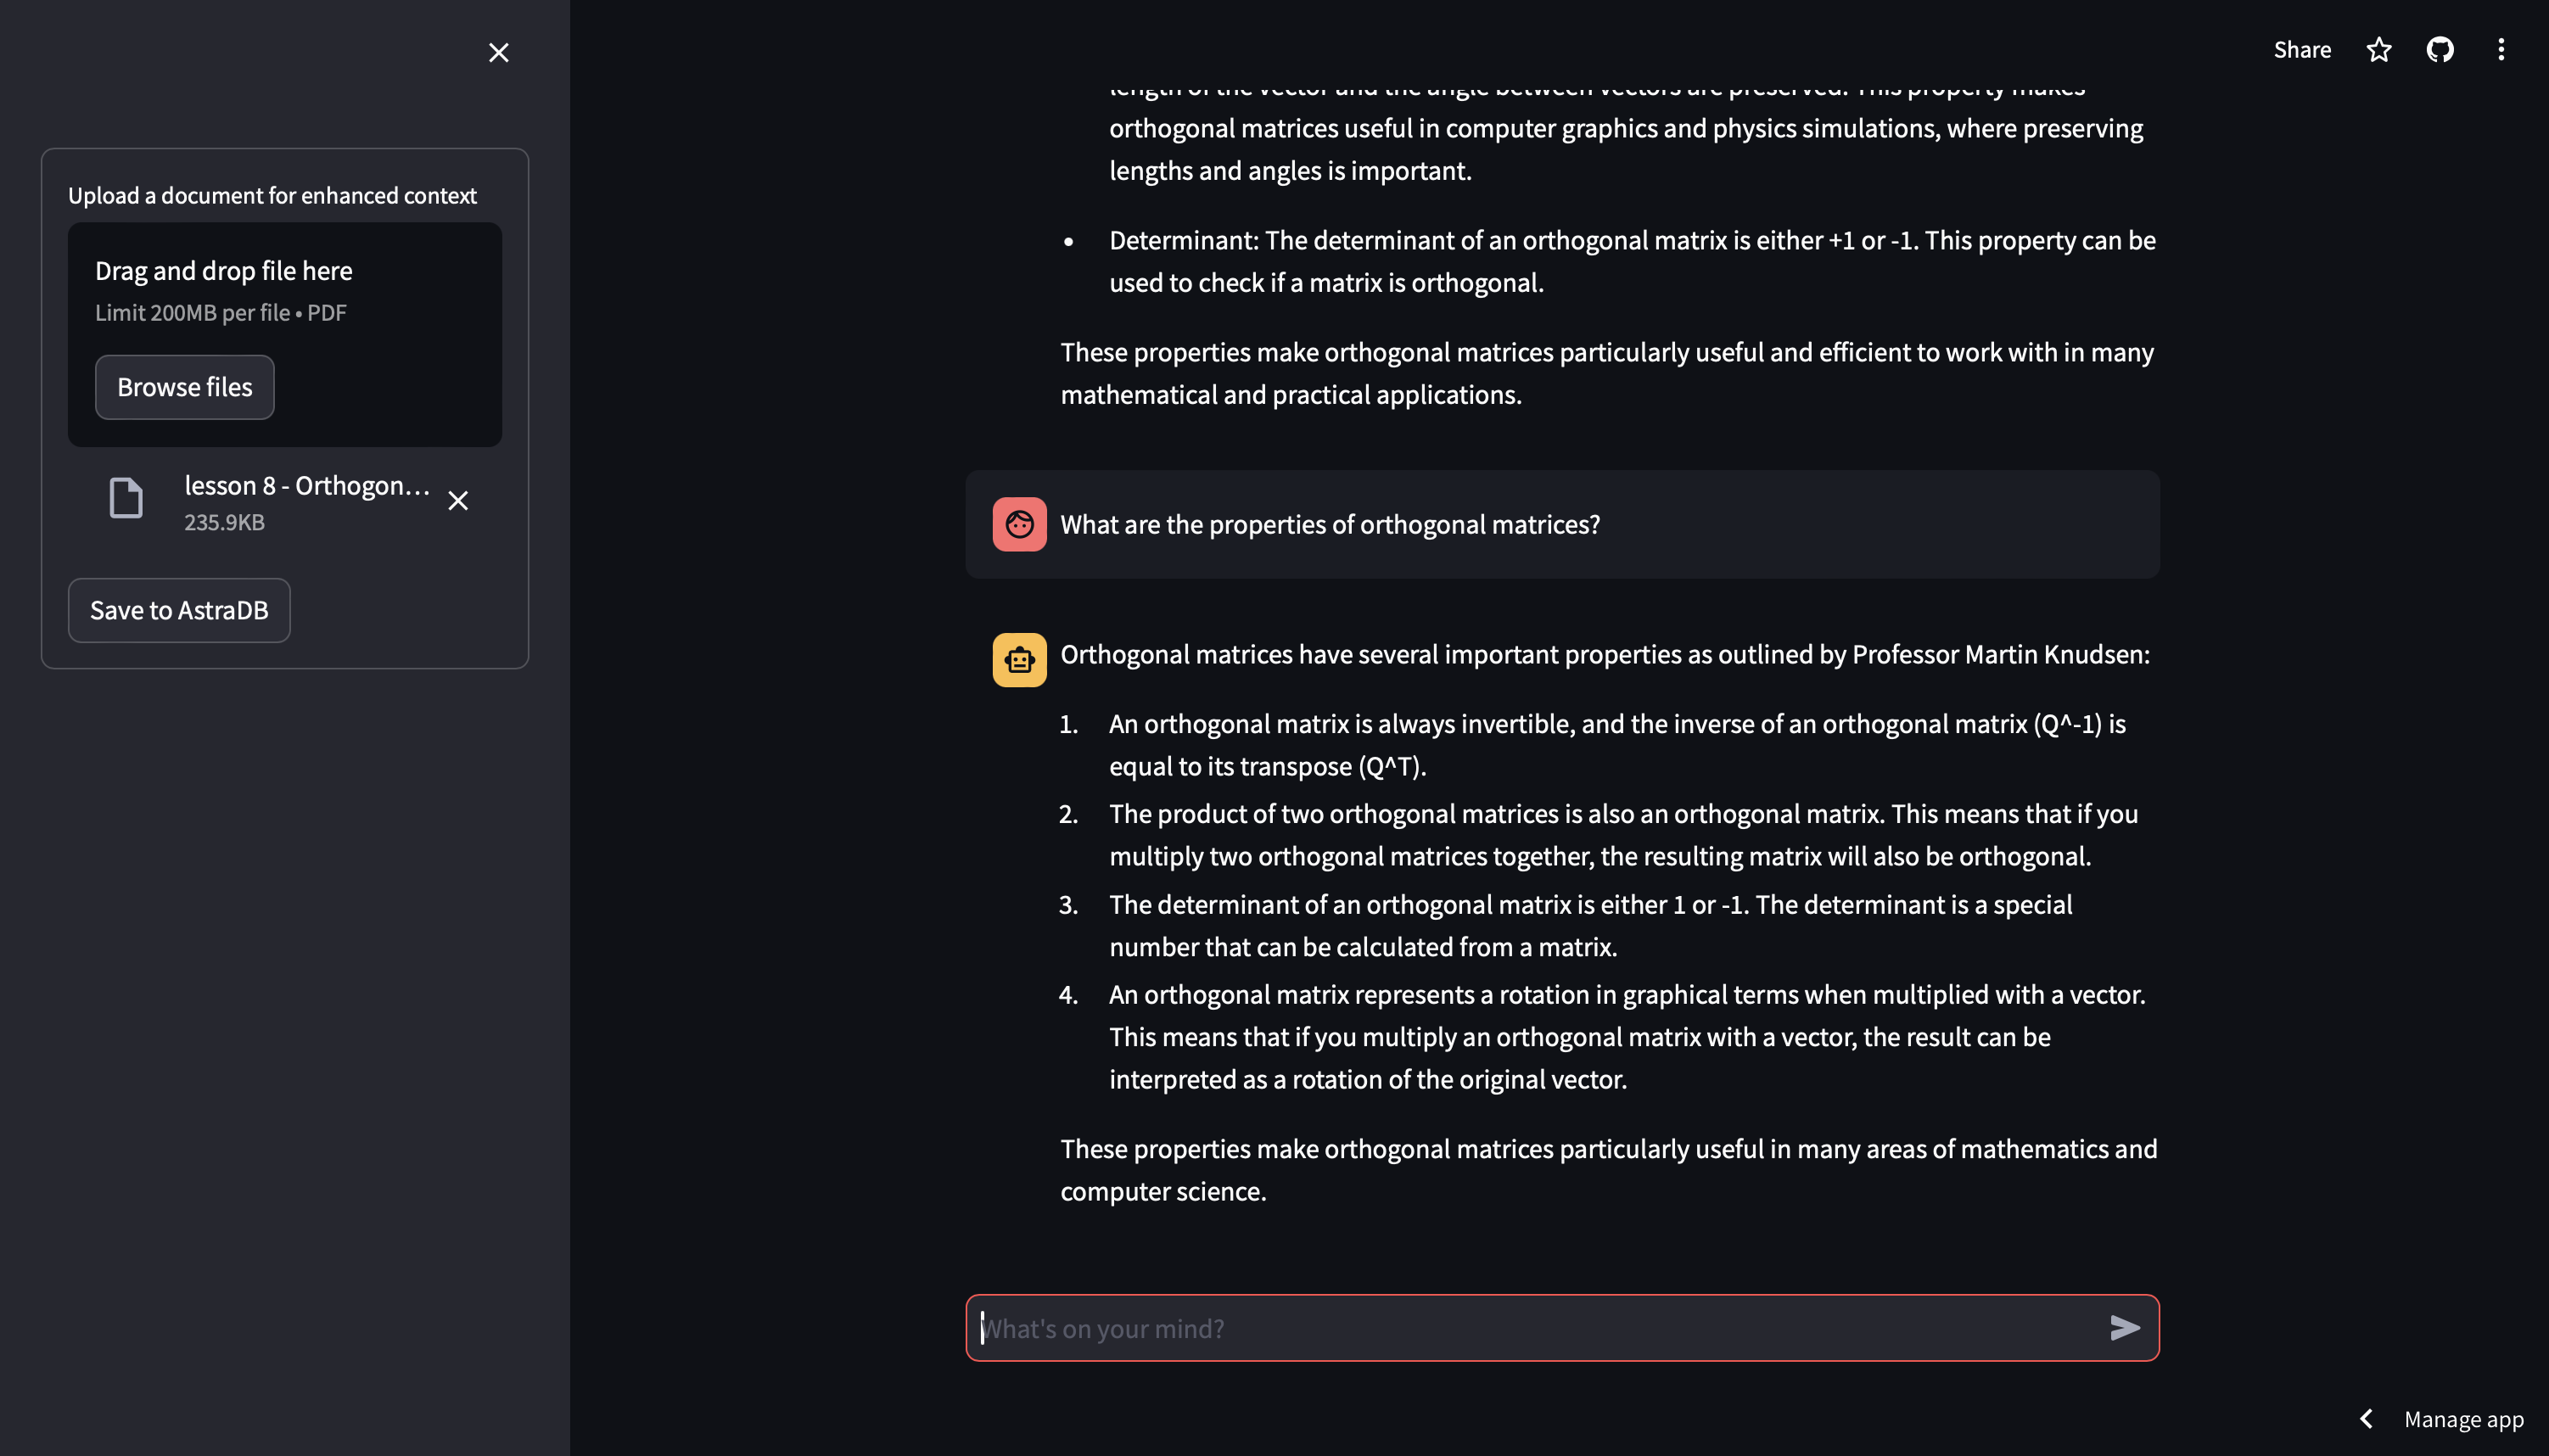
\includegraphics[width=0.8\textwidth]{figs/AfterOrthogonal.png}
        \caption{Response after insertion of lecture slides on orthogonal matrices}
        \label{fig:after_orthogonal_matrices}
    \end{figure}
    In this case we see that the professor who created the slides was referenced in the response, which was not present in the response before the document insertion. Furthermore, the response is almost identical in both structure and wording to one of the slides in the uploaded document.
\end{itemize}

\textbf{Example Query 2:}\label{uncommon_topic}
The second query was related to an uncommon topic, e.g. a project I did earlier in my studies, and involved asking the chatbot to explain the purpose of the system developed during the project. This query was chosen to test the chatbot's ability to provide information on topics that OpenAI's GPT-4 model is not familiar with.
\begin{itemize}
    \item \textbf{Before Document Insertion:} A response was produced but lacked detailed information and context about the project. 
    \begin{figure}[H]
        \centering
        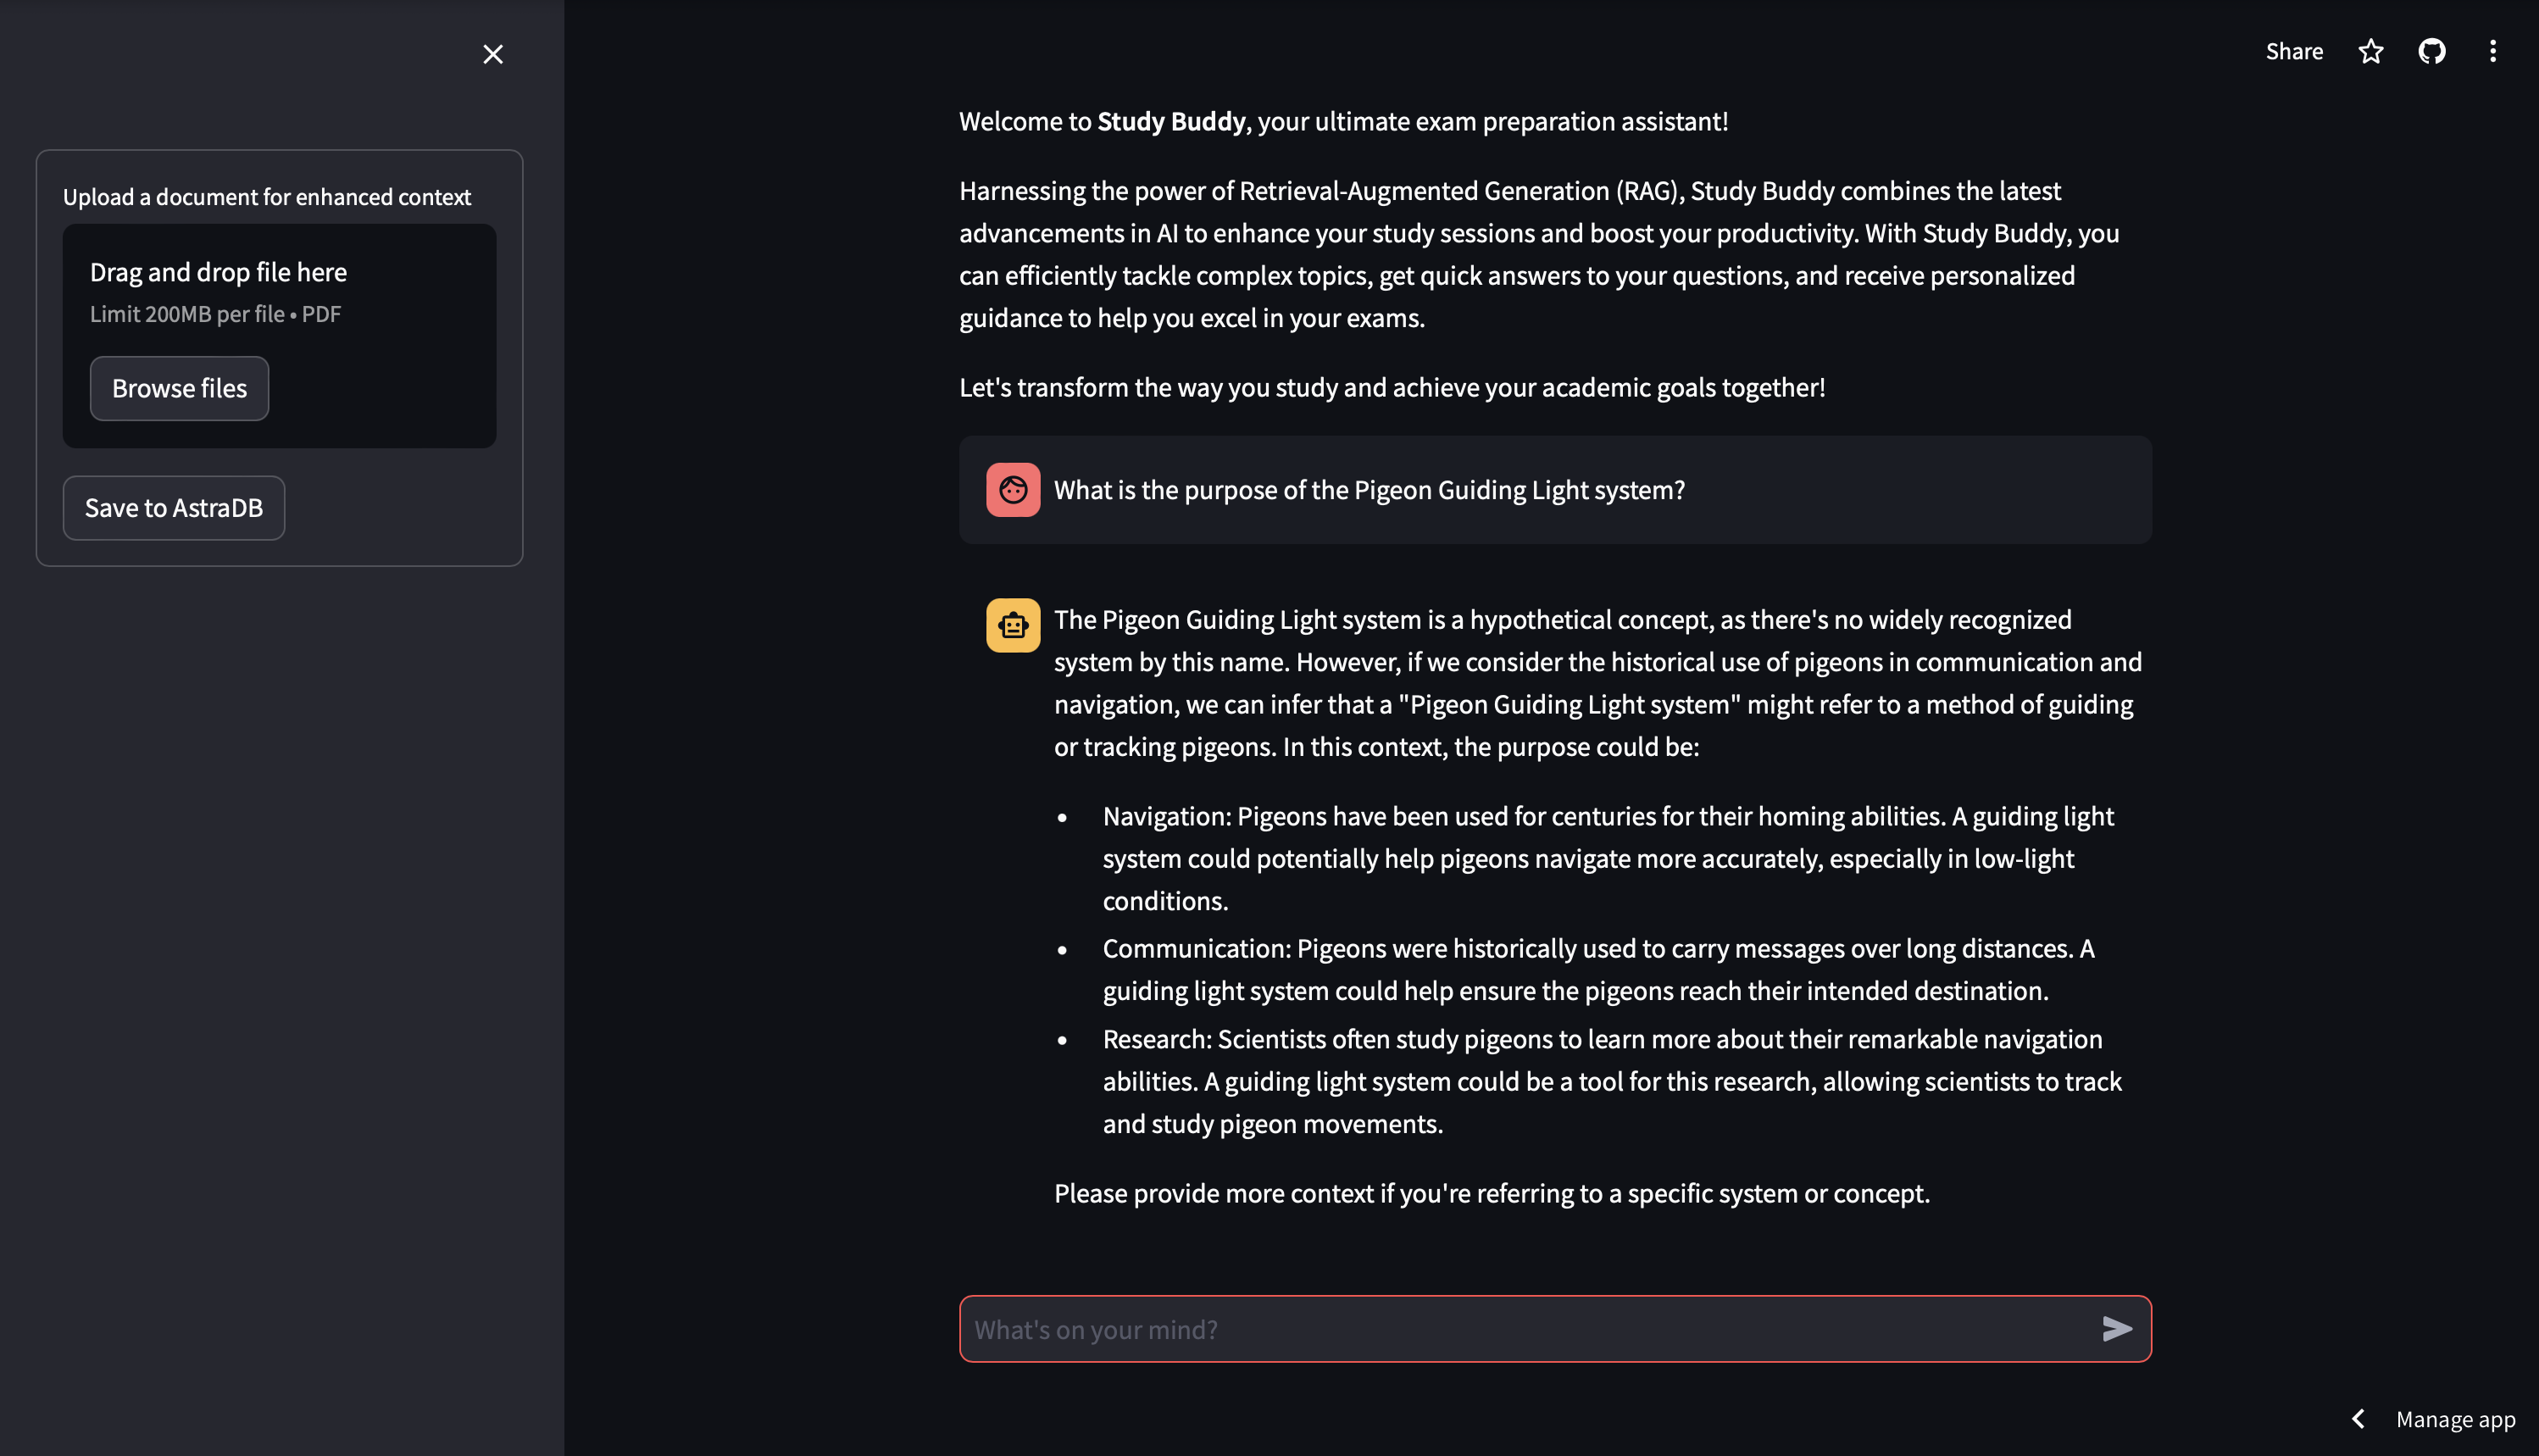
\includegraphics[width=0.8\textwidth]{figs/BeforePGL.png}
        \caption{Response before insertion of project documentation}
        \label{fig:before_project}
    \end{figure}
    \item \textbf{After Document Insertion:} The response included a detailed explanation in bullet points of the project, providing fast insight to a project that is not accesible for ChatGPT-4.
    \begin{figure}[H]
        \centering
        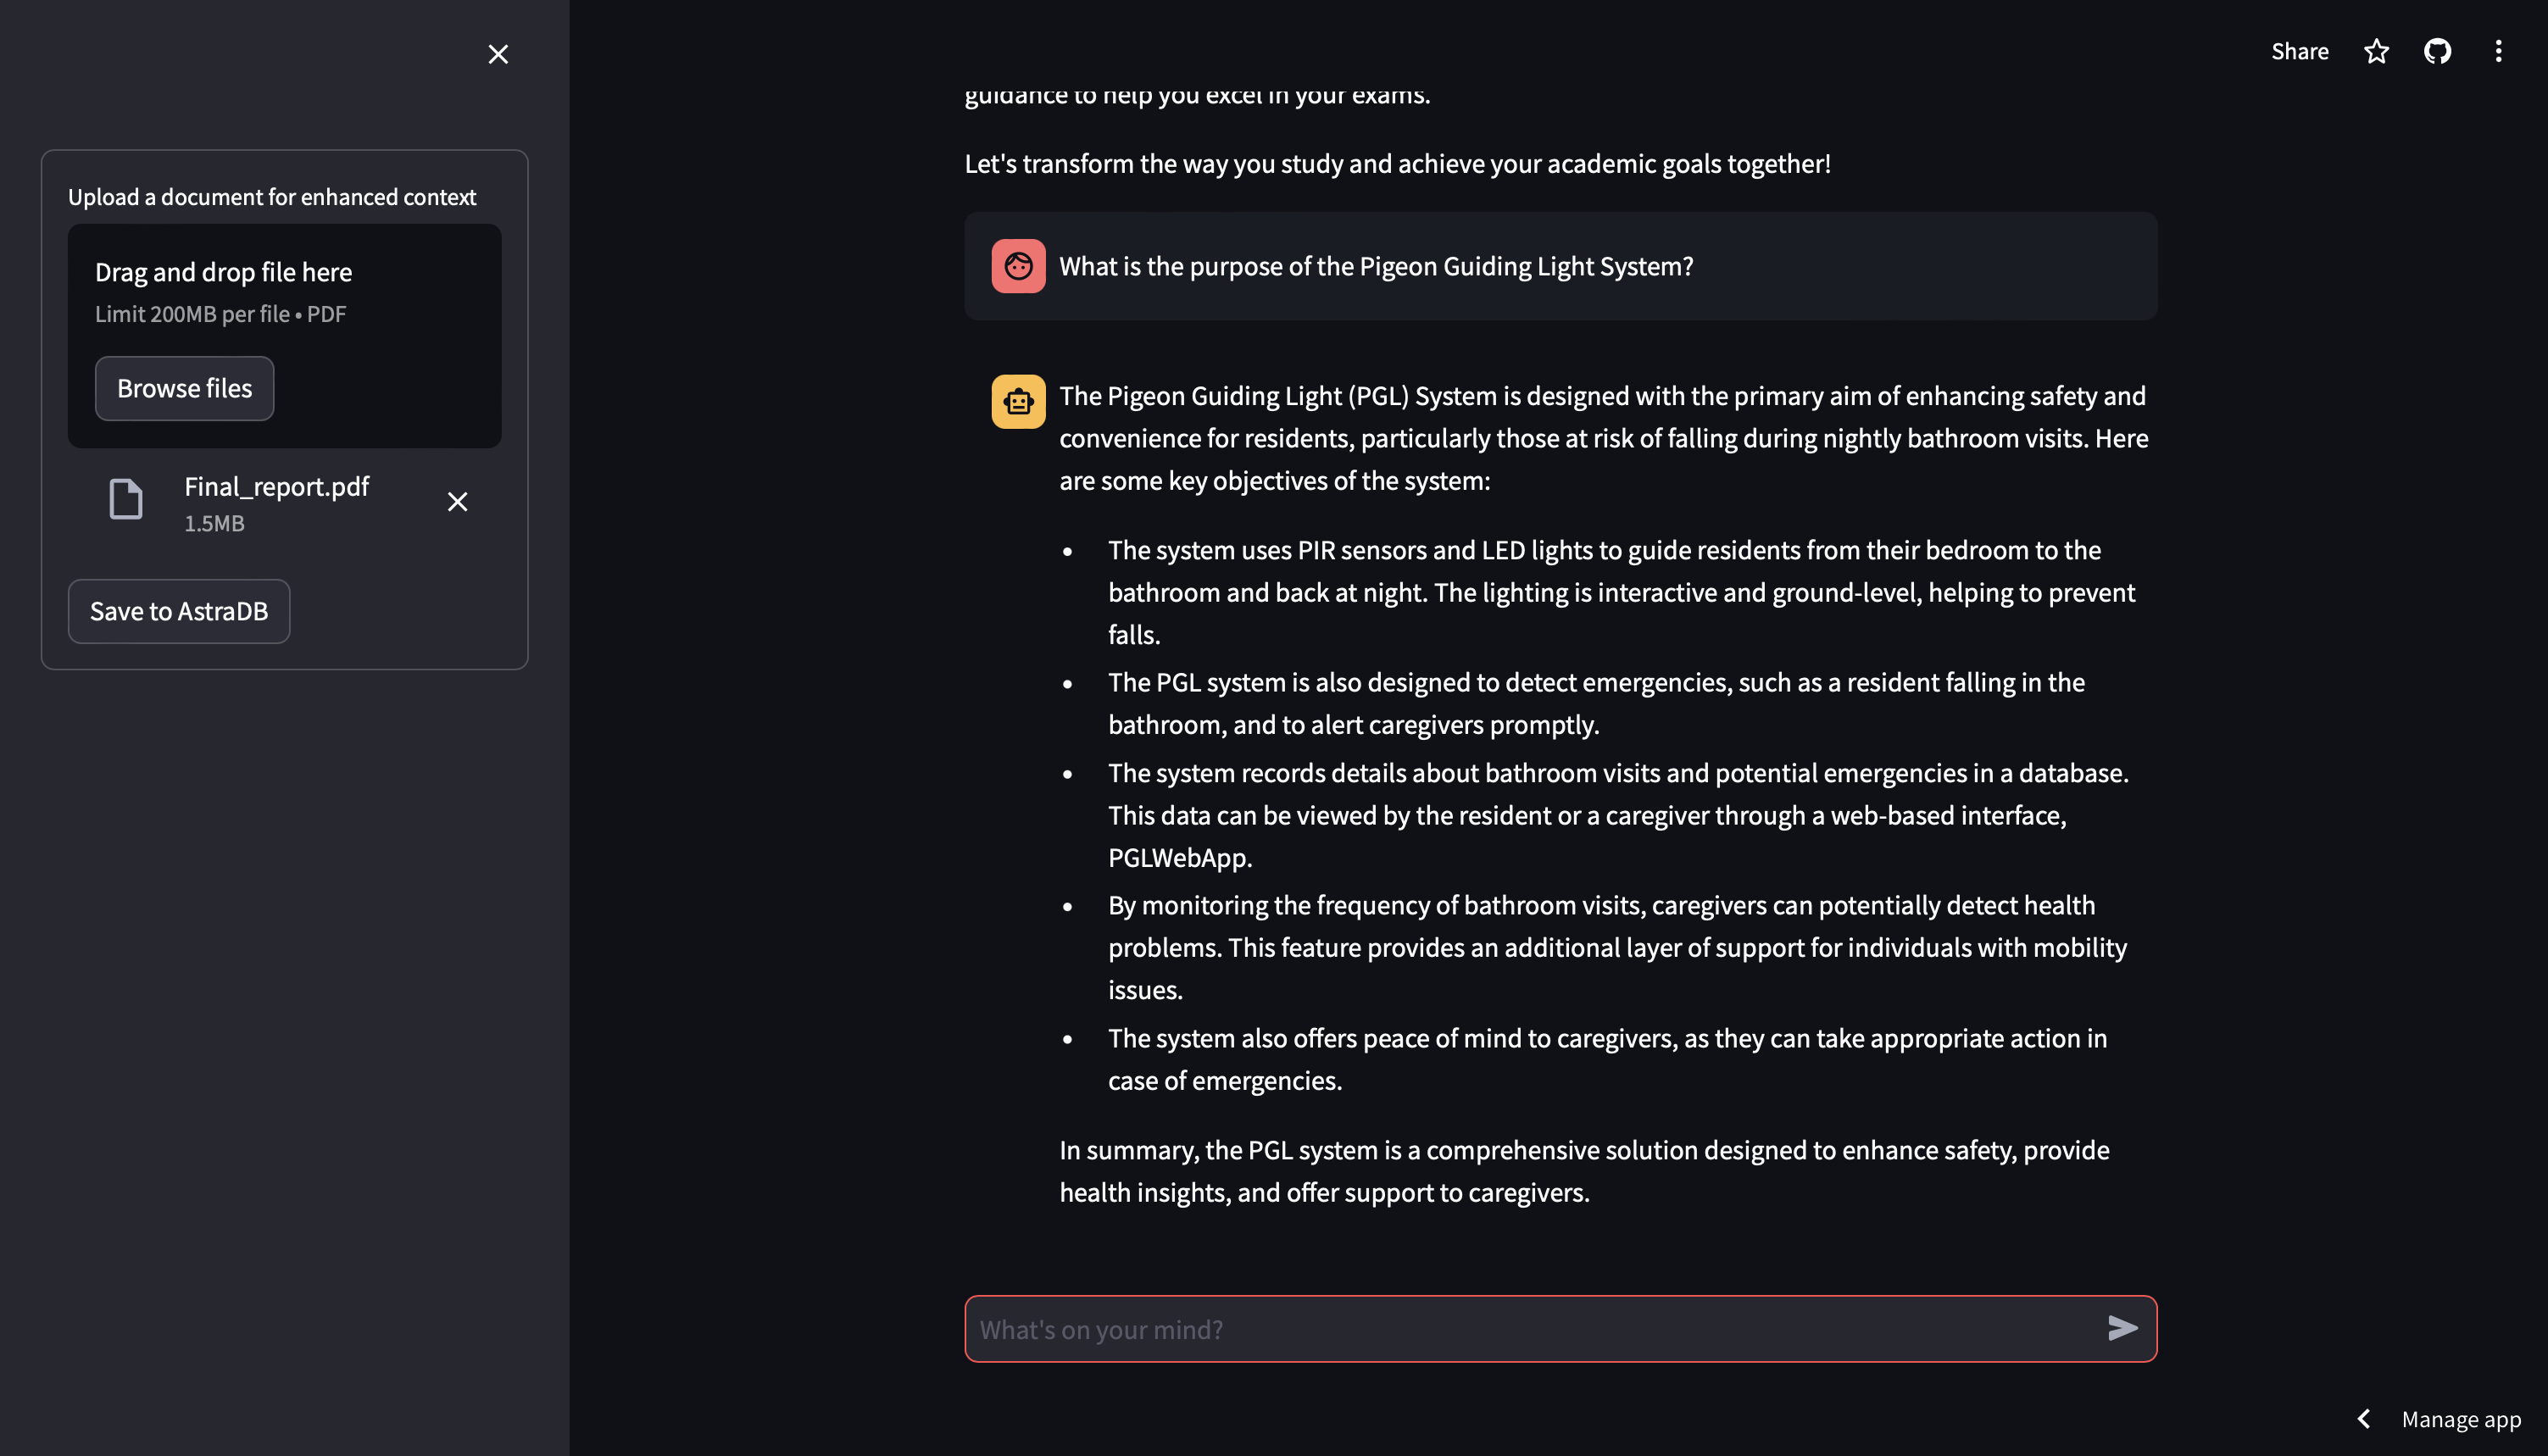
\includegraphics[width=0.8\textwidth]{figs/AfterPGL.png}
        \caption{Response after insertion of project documentation}
        \label{fig:after_project}
    \end{figure}
\end{itemize}

\subsection{Case Study: Impact of Document Insertion on Unrelated Query Response} \label{unrelated_query}
\begin{itemize}
    \item \textbf{Document Insertion of a Single Document:} After inserting only a document on "orthogonal matrices," a query was made on a different topic, e.g. "eigenvectors". The chatbot was not able to provide a relevant response, indicating that the document insertion did impact the chatbot's ability to respond to unrelated queries.
    \begin{figure}[H]
        \centering
        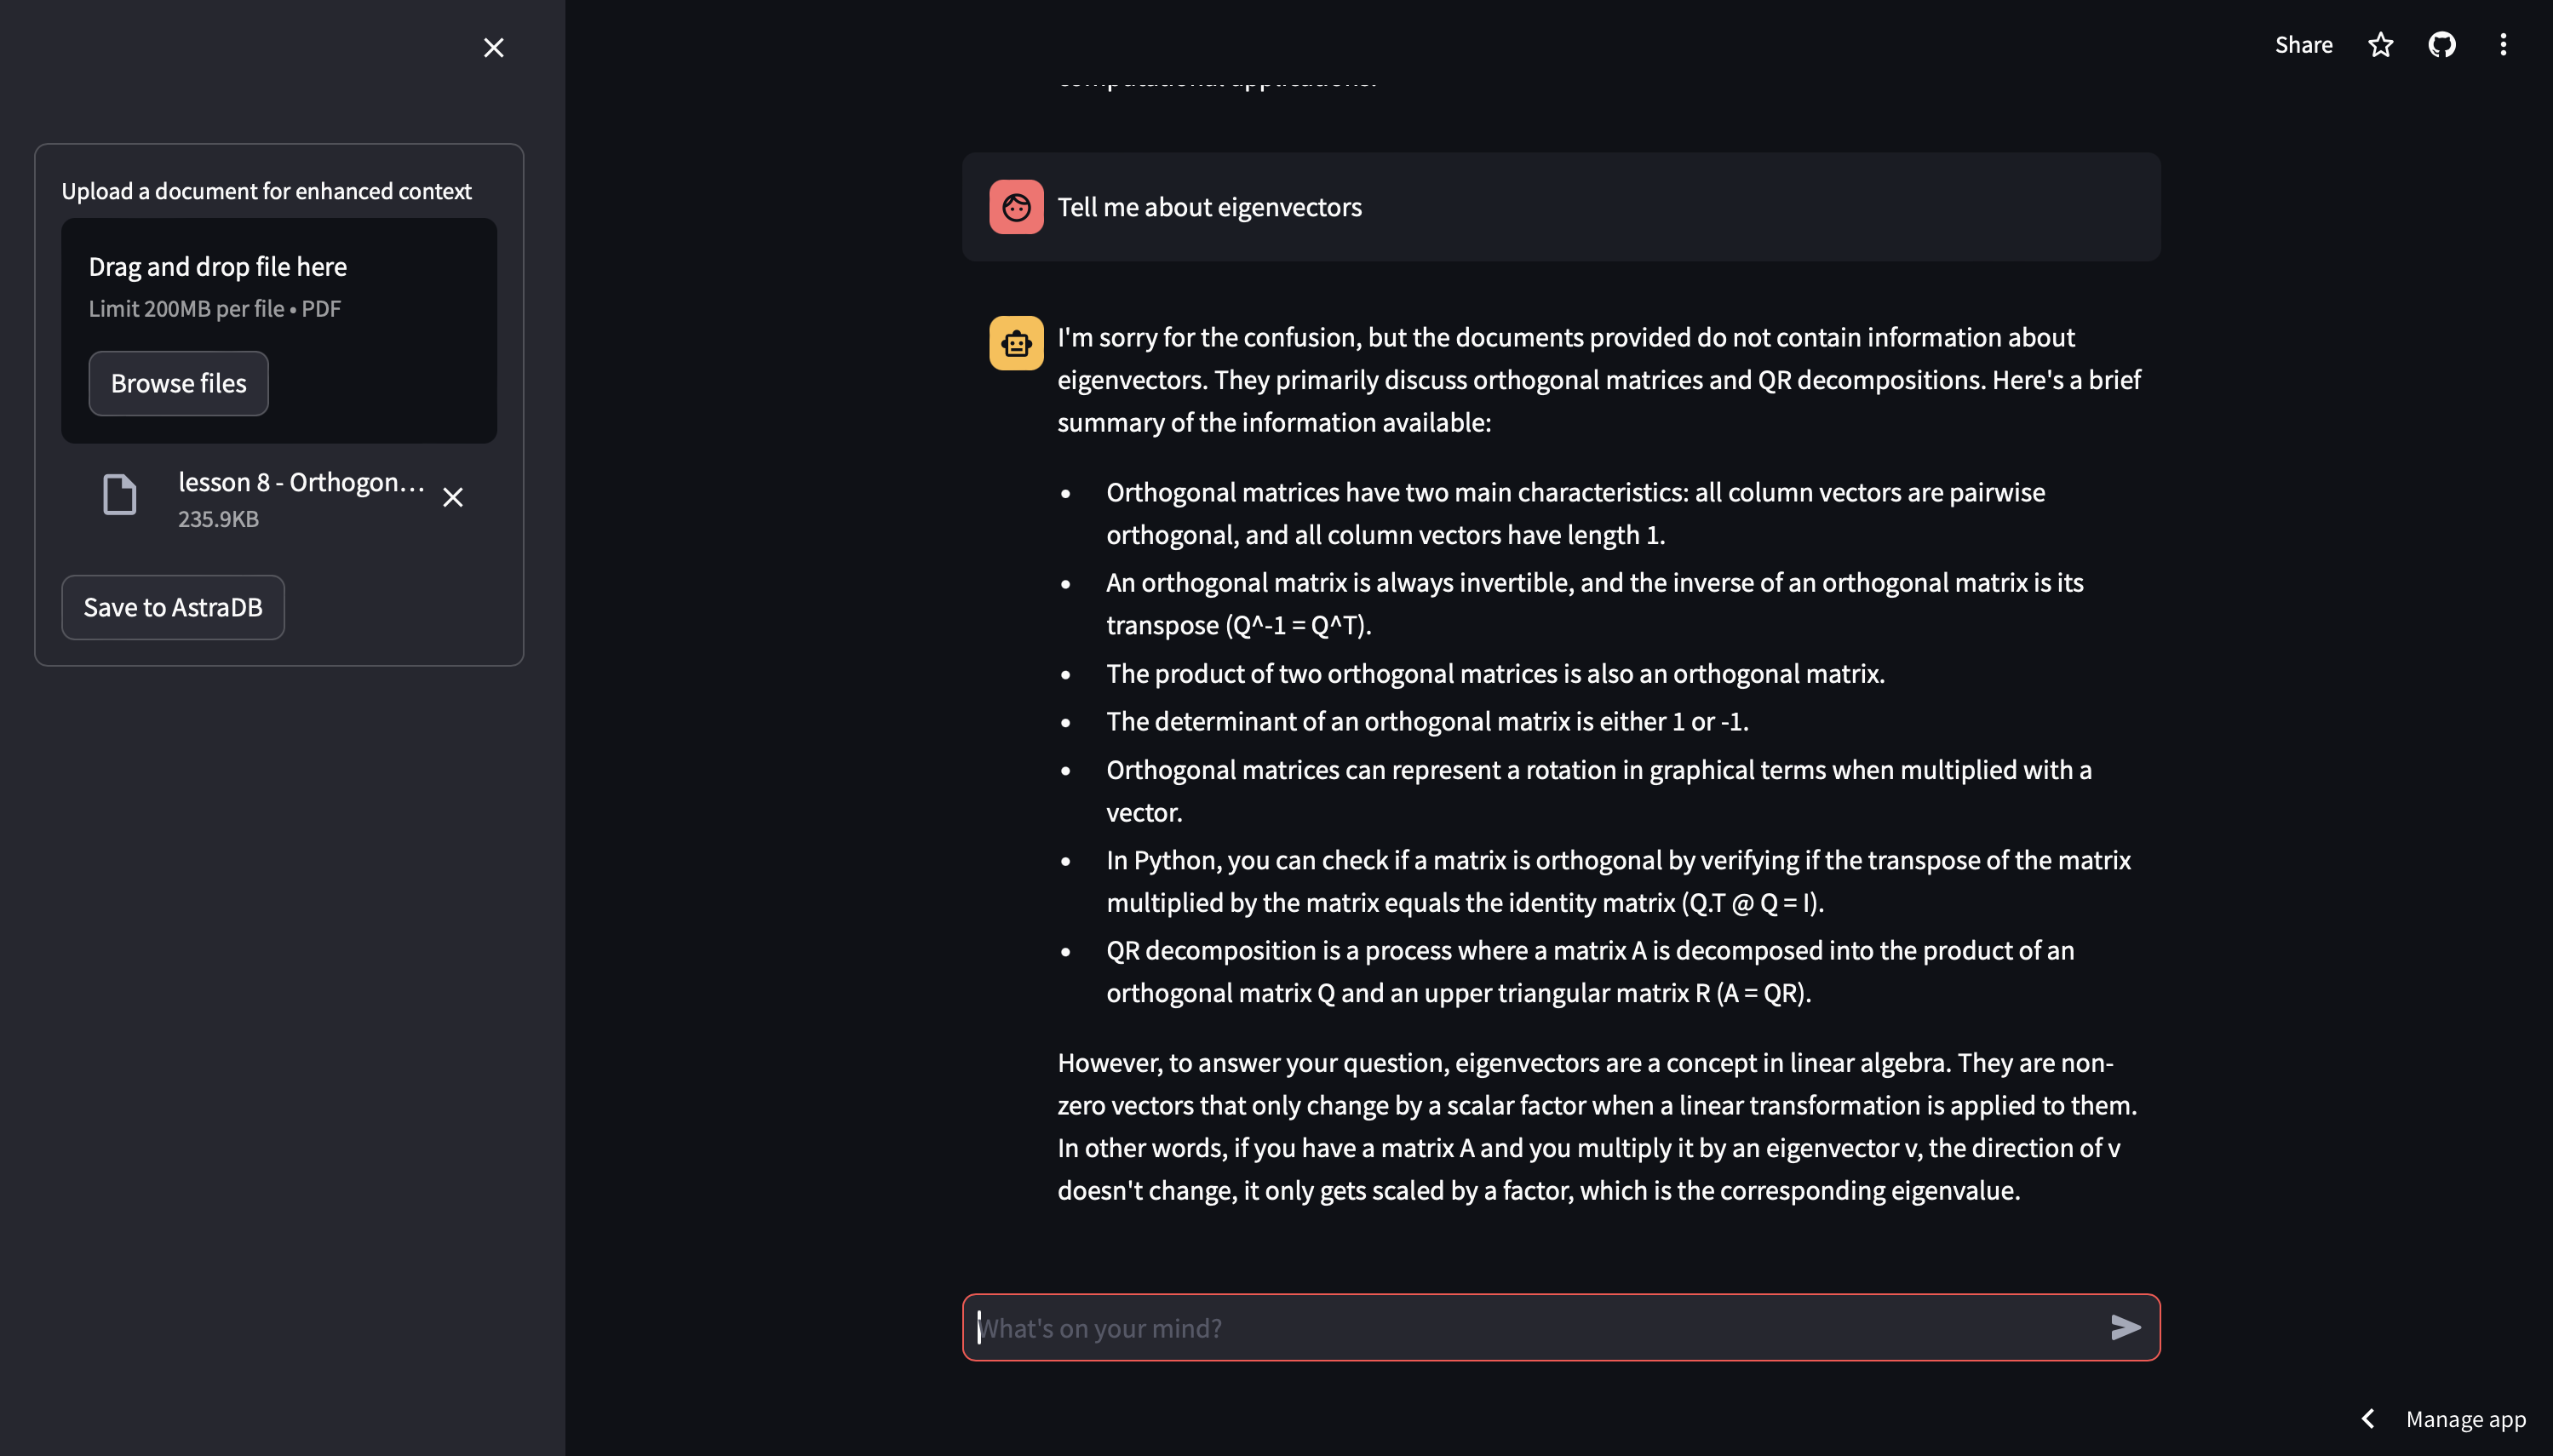
\includegraphics[width=0.8\textwidth]{figs/eigvectors.png}
        \caption{Response to an unrelated query after insertion of orthogonal matrices slides}
        \label{fig:unrelated_query}
    \end{figure}

    \item \textbf{Document Insertion of Multiple Documents:} After inserting another document on "eigenvectors," the chatbot was able to provide a relevant response to the same query on "eigenvectors." This demonstrates that the chatbot's ability to respond to queries on different topics can be improved by inserting the relevant documents.
    \begin{figure}[H]
        \centering
        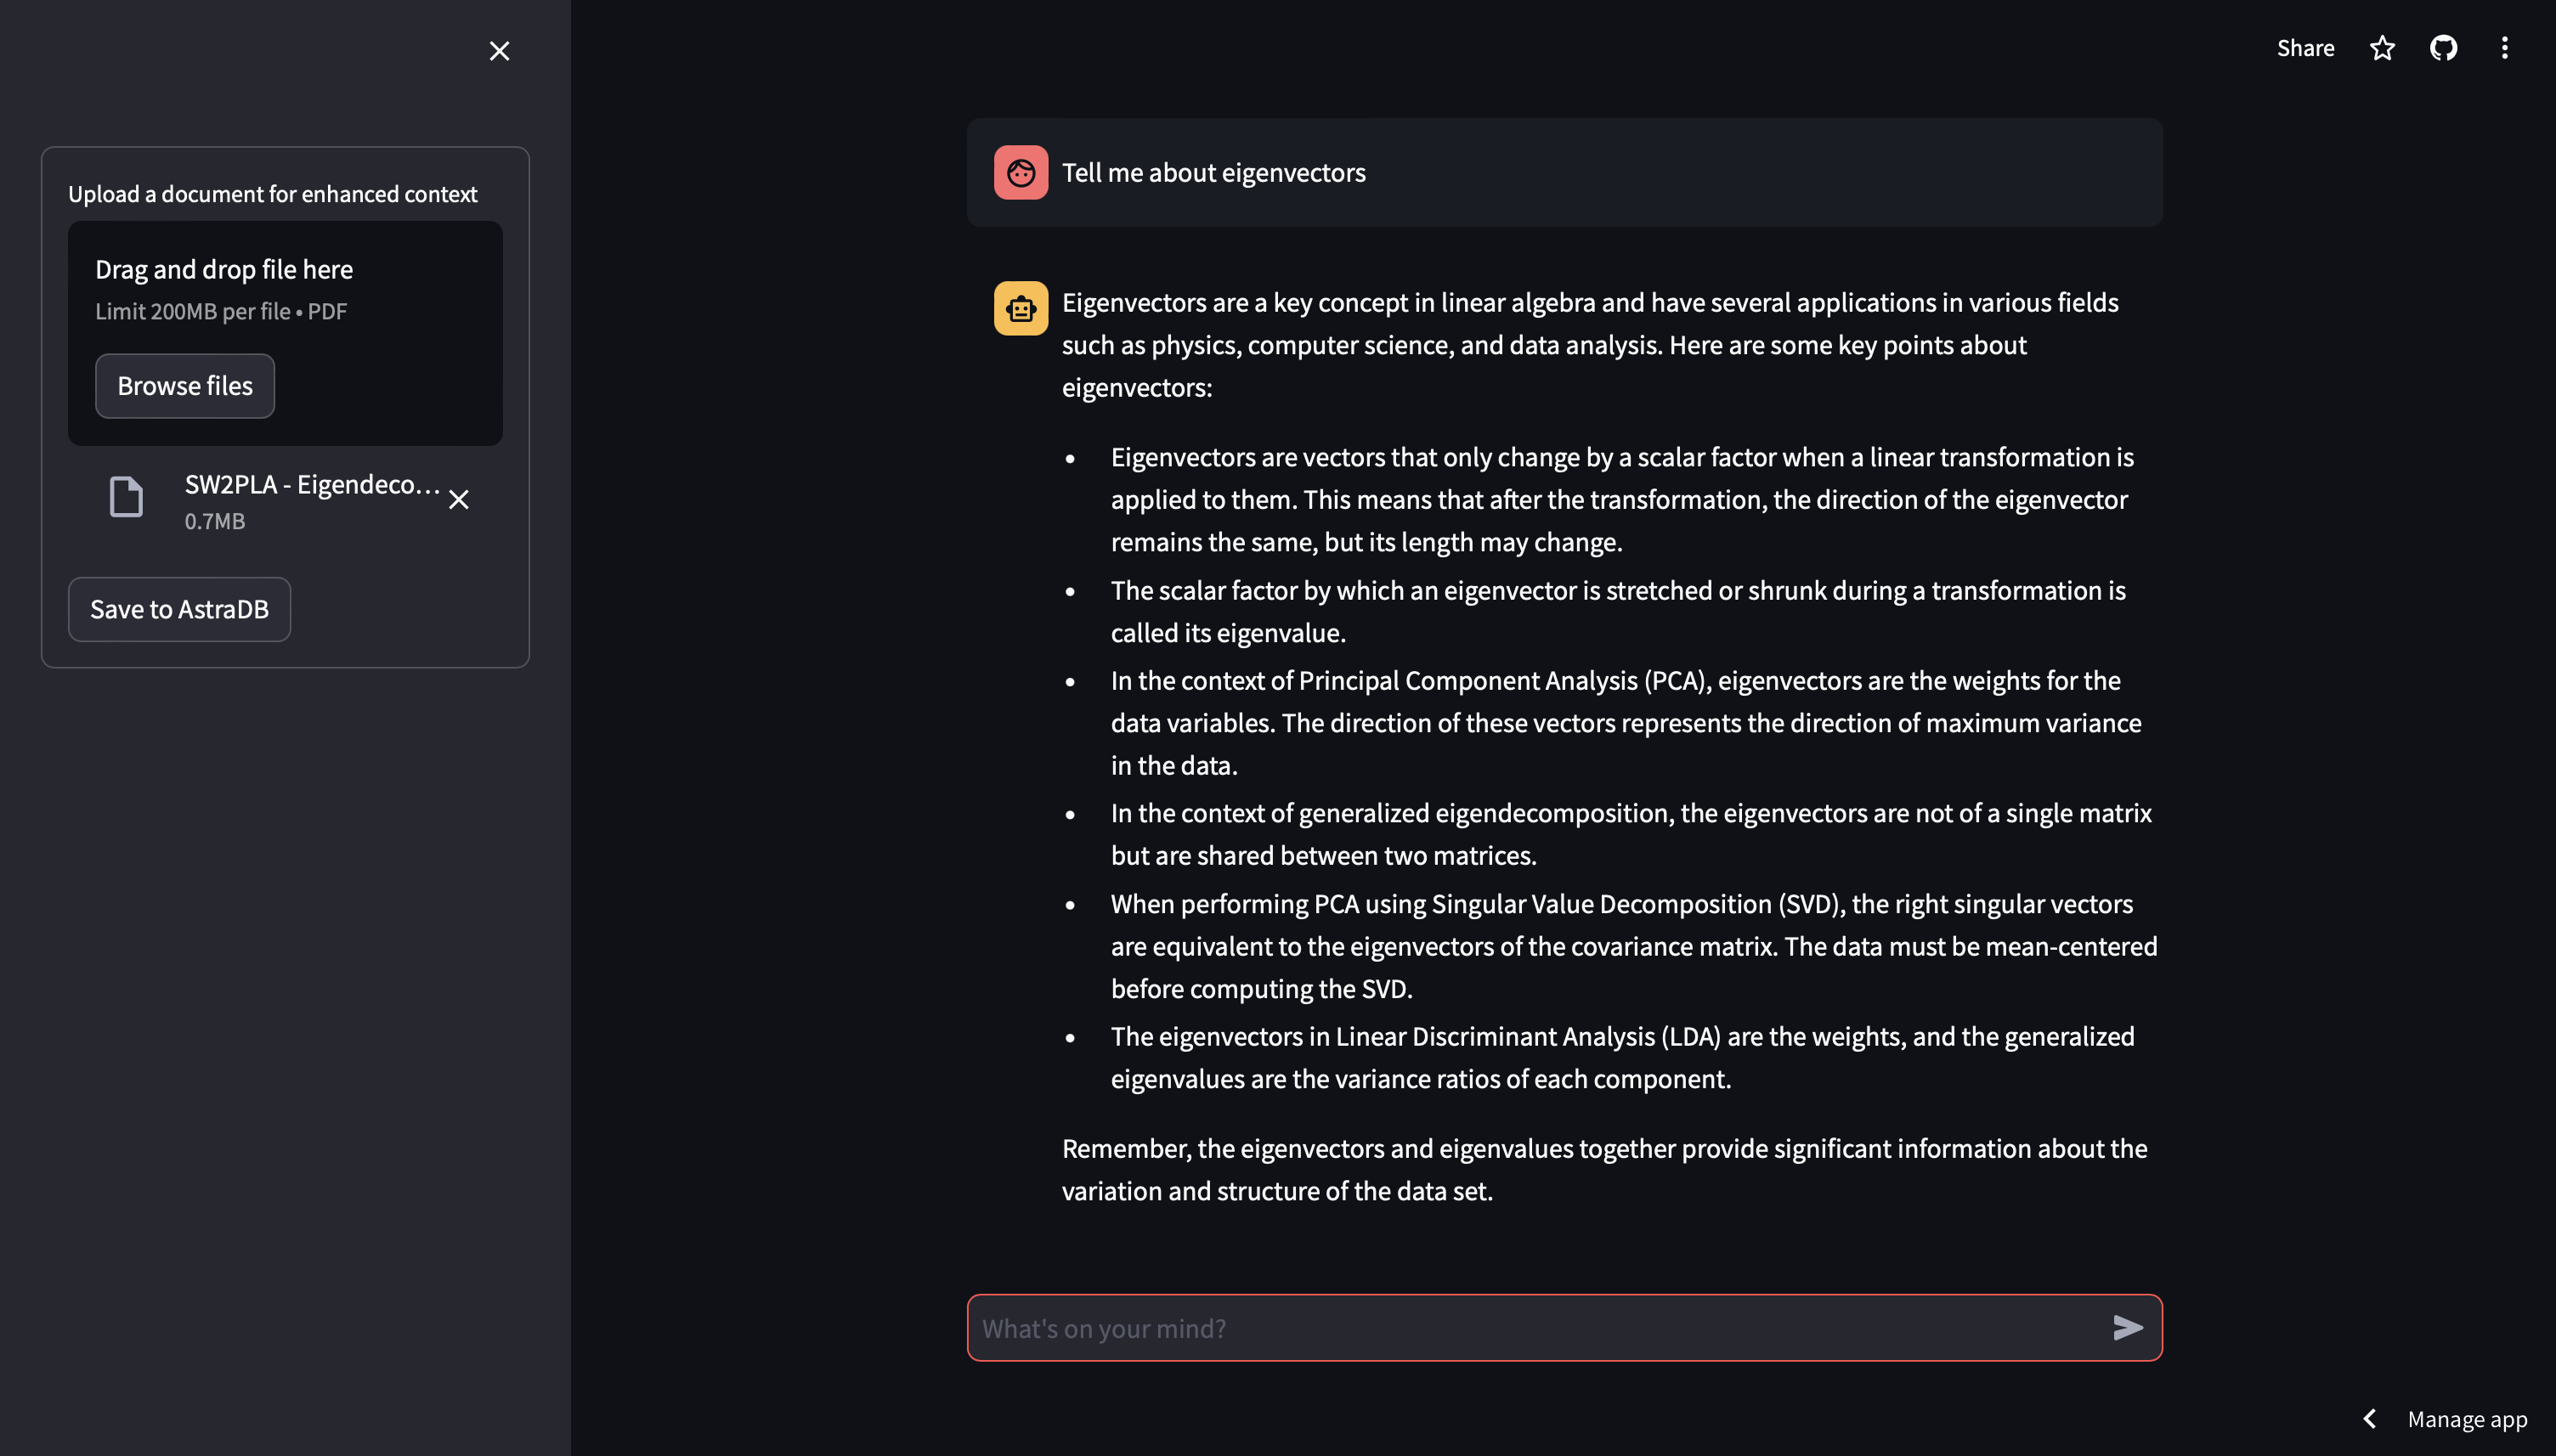
\includegraphics[width=0.8\textwidth]{figs/eigvectors2.png}
        \caption{Response to query after insertion of eigenvectors slides}
        \label{fig:unrelated_query2}
    \end{figure}
    It should be noticed that the response is tailored after the inserted document, such that it also covers PCA and SVD, which are specifically stated as related topics in the slides.
\end{itemize}
%---------------------------------------------------------------------------------------------------------------------------------------------------------------------------------------------------------------------------------------------------------------------------------

\section{Case Study: Low Rank Approximation of BART Model}
The evaluation of fine-tuning and then compressing the BART-base and BART-large model using low-rank approximation reveals the following:

\subsection{Fine-tuning the BART Model}
The fine-tuning of the BART model on the SamSum dataset provided the following results:
\begin{table}[h!]
    \centering
    \resizebox{\textwidth}{!}{%
    \begin{tabular}{cccccccc}
        \toprule
        \textbf{Epoch} & \textbf{Training Loss} & \textbf{Validation Loss} & \textbf{Rouge1} & \textbf{Rouge2} & \textbf{Rougel} & \textbf{Rougelsum} & \textbf{Gen Len} \\
        \midrule
        0 & 1.815700 & 1.543361 & 47.514900 & 24.586800 & 40.399100 & 43.972500 & 18.091700 \\
        2 & 1.458700 & \textbf{1.489950} & 48.360500 & 25.598600 & 41.272800 & 44.942500 & 17.880200 \\
        4 & 1.266000 & 1.495493 & 48.338000 & 25.252300 & 41.116400 & 44.727300 & 18.094100 \\
        6 & 1.123200 & 1.523768 & 48.887200 & 25.618700 & 41.335700 & \textbf{45.155400} & 18.206600 \\
        8 & 1.041000 & 1.528558 & \textbf{49.063600} & \textbf{25.955900} & \textbf{41.537300} & 45.311800 & \textbf{18.343500} \\
        9 & \textbf{1.019900} & 1.539690 & 48.923000 & 25.675400 & 41.485100 & 45.143400 & 18.327600 \\
        \bottomrule
    \end{tabular}
    }
    \caption{Training and Validation Metrics of Fine-Tuning BART-base across Epochs}
    \label{tab:metrics_bart_base}
\end{table}
    The fine-tuning of BART-base with 10 epochs took approximately 1 hour. It can be observed from Table \ref{tab:metrics_bart_base} that the BART-base model achieved the best training loss, ROUGE-1, ROUGE-2, and ROUGE-L scores at epoch 8. The generated length of the summaries also peaked at epoch 8, indicating that the model performed best at this stage. The ROUGE-2 score, however, was highest at epoch 9, suggesting that the model peaked in bigram overlap at this point. The training loss decreased consistently across epochs, indicating that the model was learning from the training data.

\begin{table}[H]
    \centering
    \resizebox{\textwidth}{!}{%

    \begin{tabular}{cccccccc}
    \toprule
    \textbf{Epoch} & \textbf{Training Loss} & \textbf{Validation Loss} & \textbf{Rouge1} & \textbf{Rouge2} & \textbf{Rougel} & \textbf{Rougelsum} & \textbf{Gen Len} \\
    \midrule
    0 & 1.022900 & 1.489733 & 48.960100 & 26.305700 & 41.343800 & 44.952700 & \textbf{19.270200} \\
    2 & 1.010700 & \textbf{1.386865} & \textbf{50.152900} & \textbf{27.821400} & \textbf{43.000900} & \textbf{46.561300} & 18.358200 \\
    4 & \textbf{0.812600} & 1.429855 & 50.003400 & 26.972100 & 42.172400 & 45.977900 & 18.588000 \\
    %5 & 0.821300 & 1.438000 & 49.993300 & 27.073300 & 42.191300 & 46.003100 & 18.467800 \\
    \bottomrule
    \end{tabular}
    }
    \caption{Training and Validation Metrics of Fine-Tuning BART-large across Epochs}
    \label{tab:metrics_bart_large}
    \end{table}

    The fine-tuning of BART-large with 5 epochs took approximately 1 hour and 50 minuters. Table \ref{tab:metrics_bart_large} shows that the BART-large model achieved the best validation loss, ROUGE-1, ROUGE-2, ROUGE-L, and ROUGE-Lsum scores at epoch 2 indicating that the model performed best at this stage. The training loss decreased consistently across epochs, also indicating that the model was learning from the training data.

\subsection{ROUGE scores} The low-rank approximations upholds comparable ROUGE scores until a certain rank, after which the scores begin to decline. This indicates that the model's performance is preserved up to a certain rank, beyond which the approximation starts to impact the summarization quality. The following figures illustrate the ROUGE scores for various ranks:

\begin{figure}[H]
    \centering
    \begin{subfigure}[b]{0.45\textwidth}
        \centering
        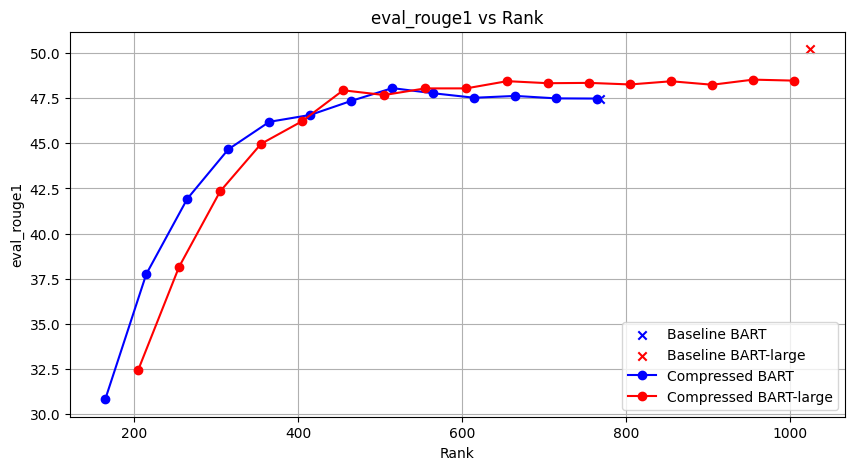
\includegraphics[width=\textwidth]{figs/06:05/Rouge1.png}
        \caption{ROUGE-1 scores.}
        \label{fig:sub1}
    \end{subfigure}
    \hfill
    \begin{subfigure}[b]{0.45\textwidth}
        \centering
        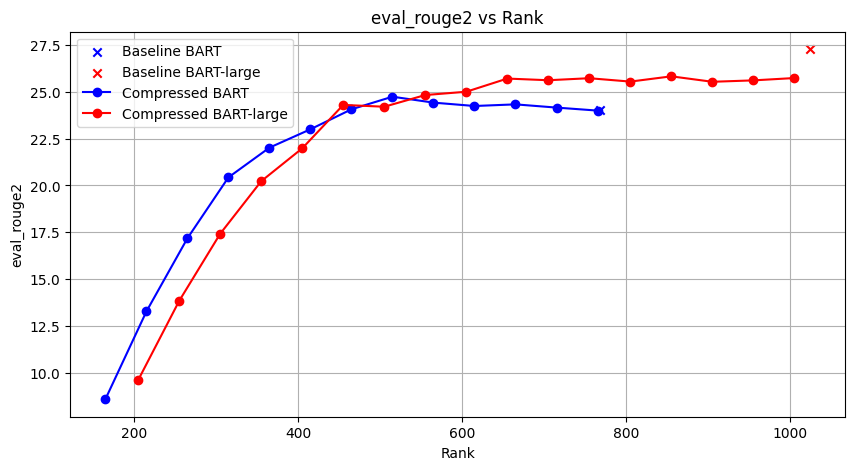
\includegraphics[width=\textwidth]{figs/06:05/Rouge2.png}
        \caption{ROUGE-2 scores.}
        \label{fig:sub2}
    \end{subfigure}
    \vskip\baselineskip
    \begin{subfigure}[b]{0.45\textwidth}
        \centering
        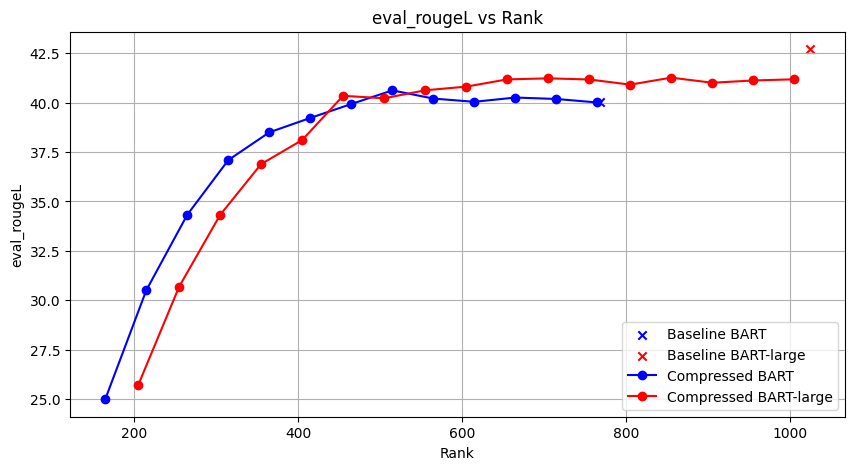
\includegraphics[width=\textwidth]{figs/06:05/RougeL.png}
        \caption{ROUGE-L scores.}
        \label{fig:sub3}
    \end{subfigure}
    \hfill
    \begin{subfigure}[b]{0.45\textwidth}
        \centering
        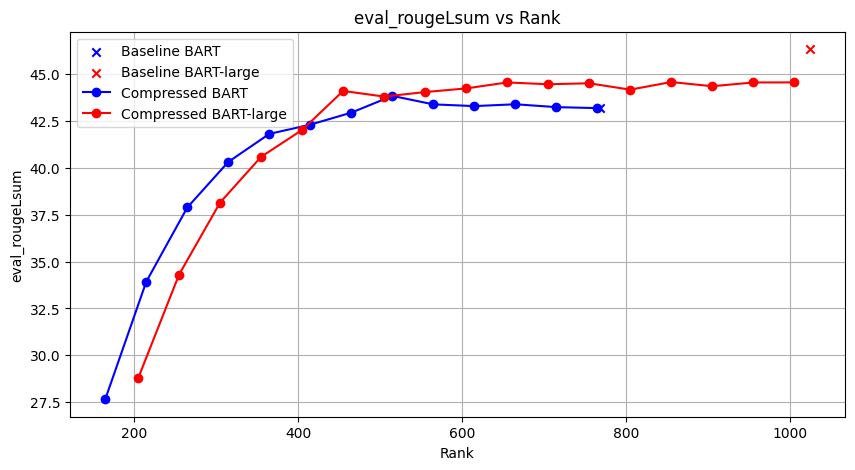
\includegraphics[width=\textwidth]{figs/06:05/RougeLSum.png}
        \caption{ROUGE-Lsum scores.}
        \label{fig:sub4}
    \end{subfigure}
    \caption{ROUGE scores for different ranks.}
    \label{fig:main}
\end{figure}

As depicted in Figure \ref{fig:main}, the ROUGE-1, ROUGE-2, ROUGE-L, and ROUGE-Lsum scores for BART-base maintain similar level of performance, compared to its original fine-tuned model, up to a rank of around \(r = 510\). However, it is important to note that for the BART-large model, there is an immediate decline in performance even when the model is low-rank approximated near full rank. Beyond that, similarly for BART-large, after the rank of around \(r = 510\), a rapid degradation in scores is observed, indicating the limitations of the low-rank approximation in preserving the model's quality.

\subsection{Computational Efficiency}
The low-rank approximation of the BART model succeeds in reducing the computational complexity and storage requirements of the model. The following figures illustrate the computational efficiency of the low-rank approximations:
\begin{figure}[h!]
    \centering
    \begin{subfigure}[b]{0.45\textwidth}
        \centering
        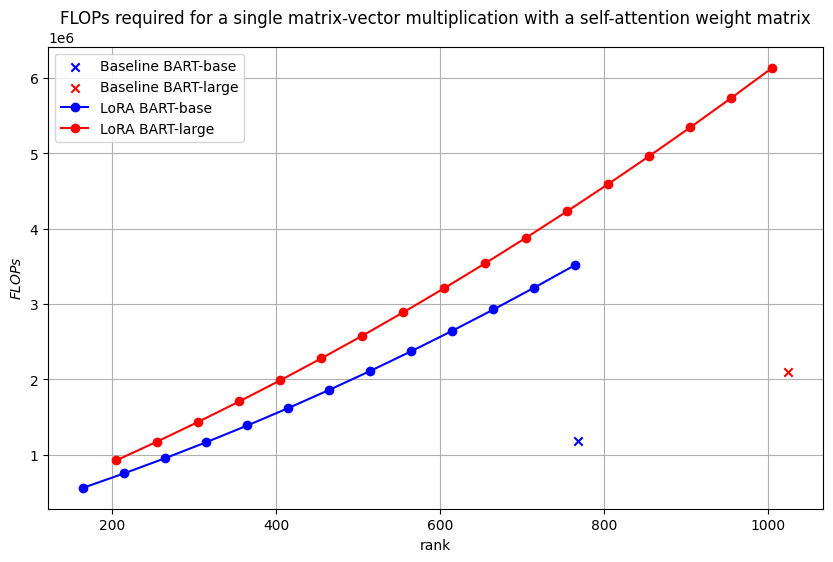
\includegraphics[width=\textwidth]{figs/flops_vector.png}
        \caption{Vector-Matrix Multiplication FLOPs.}
        \label{fig:subfigure1}
    \end{subfigure}
    \hfill
    \begin{subfigure}[b]{0.45\textwidth}
        \centering
        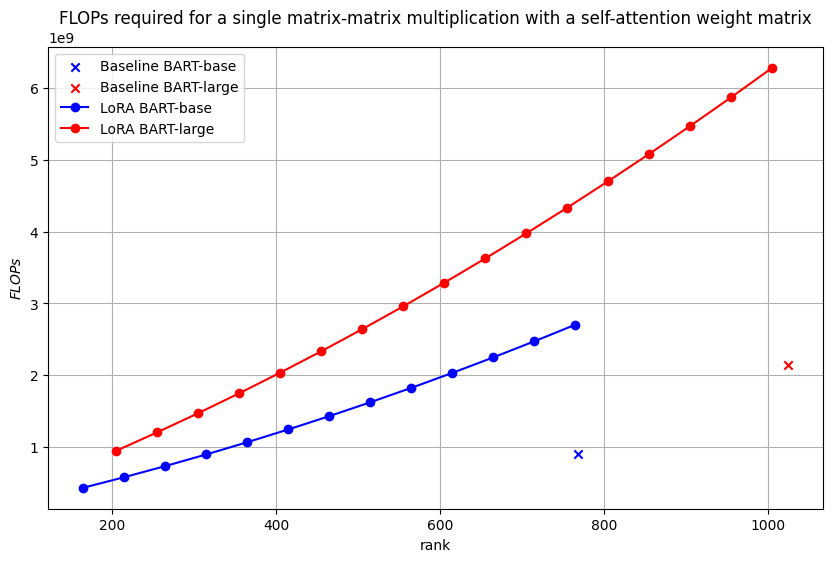
\includegraphics[width=\textwidth]{figs/flops_matrix.png}
        \caption{Matrix-Matrix Multiplication FLOPs.}
        \label{fig:subfigure2}
    \end{subfigure}
    \caption{FLOPs required for a vector-matrix multiplication and matrix-matrix multiplication of a single self-attention weight matrix in BART.}
    \label{fig:mainfigure}
\end{figure}
\begin{figure}[H]
    \centering
    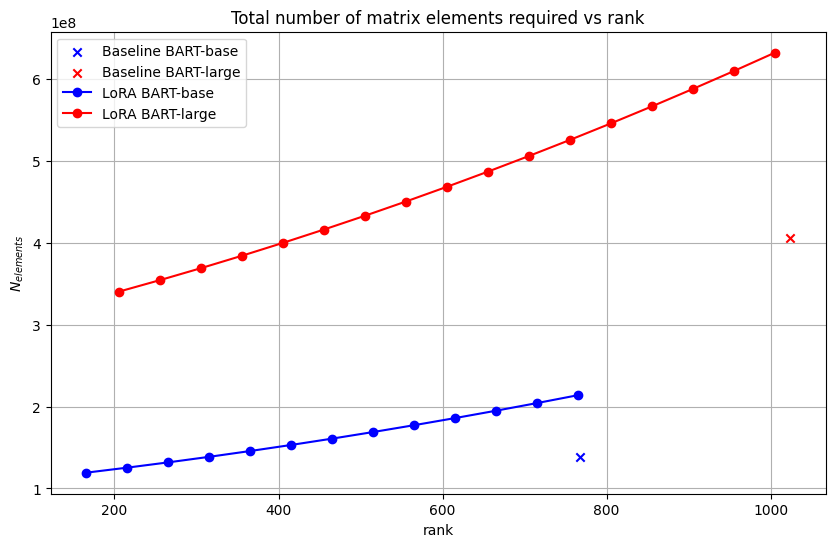
\includegraphics[width=0.6\textwidth]{figs/elements.png}
    \caption{Number of elements in the weight matrices of BART-base and BART-large depending on rank.}
    \label{fig:parameters}
\end{figure}
Figure \ref{fig:mainfigure}  show that the low-rank approximation can significantly reduce the number of FLOPs required for vector-matrix and matrix-matrix multiplications, indicating a substantial improvement in computational efficiency after a certain threshhold of \(r = 318\) and \(r = 424\) for BART-base and BART-large, respectively. The number of elements in the weight matrices of BART-base and BART-large also decreases with the reduction in rank after the same threshhold, further demonstrating the efficiency gains achieved through low-rank approximation as depicted in figure \ref{fig:parameters}.

\subsection{Comparing Summaries}

The analysis of summaries produced by the BART-base model at various ranks demonstrates how low-rank approximation affects the quality of generated summaries. \\
The following example illustrates summaries generated at different ranks: \\
At full rank (\(r_{\text{out}} = 768, r_{v} = 767, r_{k} = r_{q} = 766\)), both with and without the application of \texttt{LoRA\_Transform}, the summary is as follows:
\begin{quote}
\textit{Hannah is looking for Betty's number. Amanda can't find it. Larry called her last time they were at the park together.}
\end{quote}
While this summary differs from the reference summary (see Figure \ref{fig:SamSum_Example}), it still captures the essence of the dialogue. For simplicity let us call this the \emph{original phrasing} as we wish to compare the summaries to this as we reduce the rank.\\

The quality of the generated summaries demonstrates a noticeable decline as the rank of the low-rank approximation decreases. Initially, at higher ranks close to full rank, the summaries remain somewhat coherent and consistent, closely matching the original summary at full rank. However, as the rank decreases to \(r = 510\), the summaries start to lose details and exhibit increased errors and inconsistencies.

At ranks 765 through 730, the summary remains consistent:
\begin{quote}
    \textit{Hannah is looking for Betty's number. Amanda can't find it. Larry called her last time they were at the park together.}
\end{quote}

However, a shift is noticed at rank 725 through 720:
\begin{quote}
    \textit{Hannah doesn't know Betty's number. She texted Larry last time they were at the park together.}
\end{quote}

This slight change introduces minor variations in the narrative.

The original phrasing returns from rank 715 through 655:
\begin{quote}
    \textit{Hannah is looking for Betty's number. Amanda can't find it. Larry called her last time they were at the park together.}
\end{quote}

By rank 650 through 490, the summary shifts between losing a critical detail at times and the original phrasing:
\begin{quote}
    \textit{Hannah is looking for Betty's number. Larry called her last time they were at the park together.}
\end{quote}

As the rank decreases further, the summary begins to diverge more substantially:
\begin{quote}
    Rank 485: \textit{Amanda can't find Betty's number. Hannah doesn't know Larry.}
\end{quote}
\begin{quote}
    Rank 470: \textit{Betty's number is not in Hannah's phone.}
\end{quote}

By the time the rank reaches around 450, the summaries are severely affected:
\begin{quote}
    Rank 435: \textit{Hannah has Betty's number. She texted Larry last time they were at the park together.}
\end{quote}

Further reduction in rank leads to highly inconsistent and erroneous summaries:
\begin{quote}
    Rank 325: \textit{Amanda can't find Betty's number. Hannah and Amanda don't know each other.}
\end{quote}
\begin{quote}
    Rank 310: \textit{Amanda and Hannah don't know each other.}
\end{quote}

At the lowest ranks, the summaries become almost nonsensical:
\begin{quote}
    Rank 205: \textit{Amanda, Hannah and Amanda are going to meet up with Larry.}
\end{quote}
\begin{quote}
    Rank 175: \textit{Amanda and Amanda don't know each other person in the park.}
\end{quote}
\begin{quote}
    Rank 150: \textit{Amanda and Amanda are going to the park.}
\end{quote}

These observations further indicates that the low-rank approximation method can maintain summarization quality up to a certain rank, beyond which the coherence and accuracy of the summaries degrade significantly. This highlights the trade-off between computational efficiency and model performance in the context of low-rank approximation of the BART model.

